\scanpage{37}
Si $a$ est le pt de $S$ en dessous de $t$, et si $F_a$ est \uline{représentable par} $X_a$ \deleted{\unsure{loc.}} loc. de type fini sur $S_a$, \deleted{\unsure{fini si}} alors $\eta$ définit $u:T\mathbin{-}X_a$, posant $x=u(t)$, d'où $\bar\eta:\mathcal O_{X_a,x}\mathbin{-}\mathcal O_{T,t}$, le fait que $\eta$ soit modulaire \inserted{local} signifie que $\bar\eta$ est un \uline{isomorphisme}.

\uline{Re} N.B. Si $\eta\in F(T)$, $\eta'\in F(T')$ sont \unsure{modulaires} \inserted{local}, et s'il existe un diagramme commutatif (\unsure{a|6}), tel que
\[
F(j)(\eta(t))=F(j')(\eta'(t')),
\]
alors (\unsure{et alors} seulement) il existe un $S$-isom $\varphi:T\mathbin{-}T'$ tel que $\eta=F(\varphi)(\eta')$.

\figure{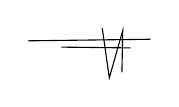
\begin{tikzpicture}[x=1cm,y=1cm]
\draw (0,0)--(1.55,.02);\draw (.42,-.08)--(1.3,-.09);\draw (.94,.16)--(1.03,-.47)--(1.2,.13)--(1.19,-.4);
\end{tikzpicture}}

\uline{Preuve prop. 3} \inserted{On peut supposer $S$ affine.} De $1^\circ)$ résulte que l'ens \deleted{de} $M(T,\eta)$ est stable par \deleted{\unsure{double}} générisation. Par $2^\circ)$, il est donc ouvert. \deleted{Donc pour $\forall$ \unsure{d'où le}} \inserted{Utilisant $\underset{\leftarrow}{L}_2$,} Pour $\forall a\in S$ et $x\in X_a$ sur $a$, \deleted{\unsure{soit}} il existe donc un \unsure{«} $X^{(*)}$ \deleted{\unsure{local}} affine, \deleted{loc.} de t. fini sur $S$, et $\eta^{(*)}\in F(X^{(*)})$, \uline{modulaire} \inserted{local} en
\mspage{36}
